\documentclass[12pt]{article}
\usepackage[spanish]{babel}

%%%%%%%%%%%%%%%%%%%%%%%%%%%%%%%%%%
%%%%%%%%%%%%%%%%%%%%%%%%%%%%%   %%
%%        Datos Trabajo     %%  %%
%%%%%%%%%%%%%%%%%%%%%%%%%%%%%%%%%%
\newcommand{\titulo}[0]{Evidencia de aprendizaje: Reporte estadístico}
\newcommand{\materia}[0]{Estadística Básica}
\newcommand{\grupo}[0]{BI-BEBA-2002-B2-013}
\newcommand{\unidad}[0]{Unidad 3}


%%%%%%%%%%%%%%%%%%%%%%%%%%%%%%%%%%
%%%%%%%%%%%%%%%%%%%%%%%%%%%%%%%%%%
\usepackage{amssymb}
\usepackage{enumerate}
\usepackage{geometry}
\usepackage{mathtools}
\usepackage{multicol}
\usepackage{soul}

\usepackage{graphicx}
	\graphicspath{ {assets/} }

\usepackage{hyperref}
	\hypersetup{
			pdftex,
		        pdfauthor={bench},
		        pdftitle={\titulo},
		        pdfsubject={\materia},
		        pdfkeywords={\grupo, \unidad, UnADM},
		        pdfproducer={Latex with hyperref, Ubuntu},
		        pdfcreator={pdflatex, or other tool},
			colorlinks=true,
				linkcolor=[rgb]{0,0,0.45},
				urlcolor=cyan,
				filecolor=green,
				citecolor=blue}

%%%%%%%%%%%%%%%%%%%%%%%%%%%%%%%%%%
%%%%%%%%%%%%%%%%%%%%%%%%%%%%%%%%%%

\title{
	
\includegraphics{../../../assets/logo-unadm} \\
	\ \\ Benjam\'in Rivera \\
	\bf{\titulo}\\\ \\}

\author{
	Universidad Abierta y a Distancia de México \\
	TSU en Biotecnolog\'ia \\
	\textit{Materia:} \materia \\
	\textit{Grupo:} \grupo \\
	\textit{Unidad:} \unidad \\
	\\
	\textit{Matricula:} ES202105994 }

\date{\textit{Fecha de entrega:} \today}


%%%%%%%%%%%%%%%%%%%%%%%%%%%%%
%%        Documento         %%
%%%%%%%%%%%%%%%%%%%%%%%%%%%%%%%
\begin{document}
\maketitle\newpage


\section{Caso de estudio}


	\par Estoy interesado en estudiar las \textbf{t\'ecnicas de repoblaci\'on de ecosistemas} usando agentes biol\'ogicos. Uno de los t\'emas de interes para poder desarrollar esta investigaci\'on es conocer las \textbf{especies por espacio geogr\'afico} que habitan. Esto es importante para poder analizar ecosistemas afectados y aquellos que sean sanos, y que posean caracteristicas similares. 

	\begin{figure}[h]
		\centering
			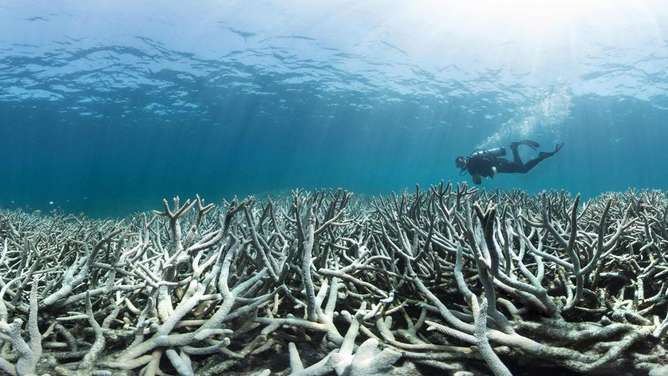
\includegraphics[width=0.6\textwidth]{coral-muerto.jpg}
		\caption{Corales muertos en el Océano Índico por culpa del calentamiento global \cite{corales muertos}}
		\label{fig: corales muertos}
	\end{figure}
	

	\par Entonces en \textbf{esta parte} nos centraremos en las \textbf{ubicaciones de los bancos de algas del mundo}. Esta informaci\'on nos pertmitira teorizar t\'ecnicas de \textit{biorremediaci\'on} en funci\'on de otros ambientes similares. Adem\'as, el estudio de estos en alg\'un tiempo determinado nos dara una oportunidad para identificar causas de infeccion y muerte de las agrupaciones de estos; para tratar de predecir los corales que esten en peligro por causas similares.
	
\section{Base de Datos}

	\par De manera que usando la base de datos \cite{db} obtenemos la visualización preliminar que podemos ver en la figura~\ref{fig: tabla}.
	
	\begin{figure}[h]
	\centering
		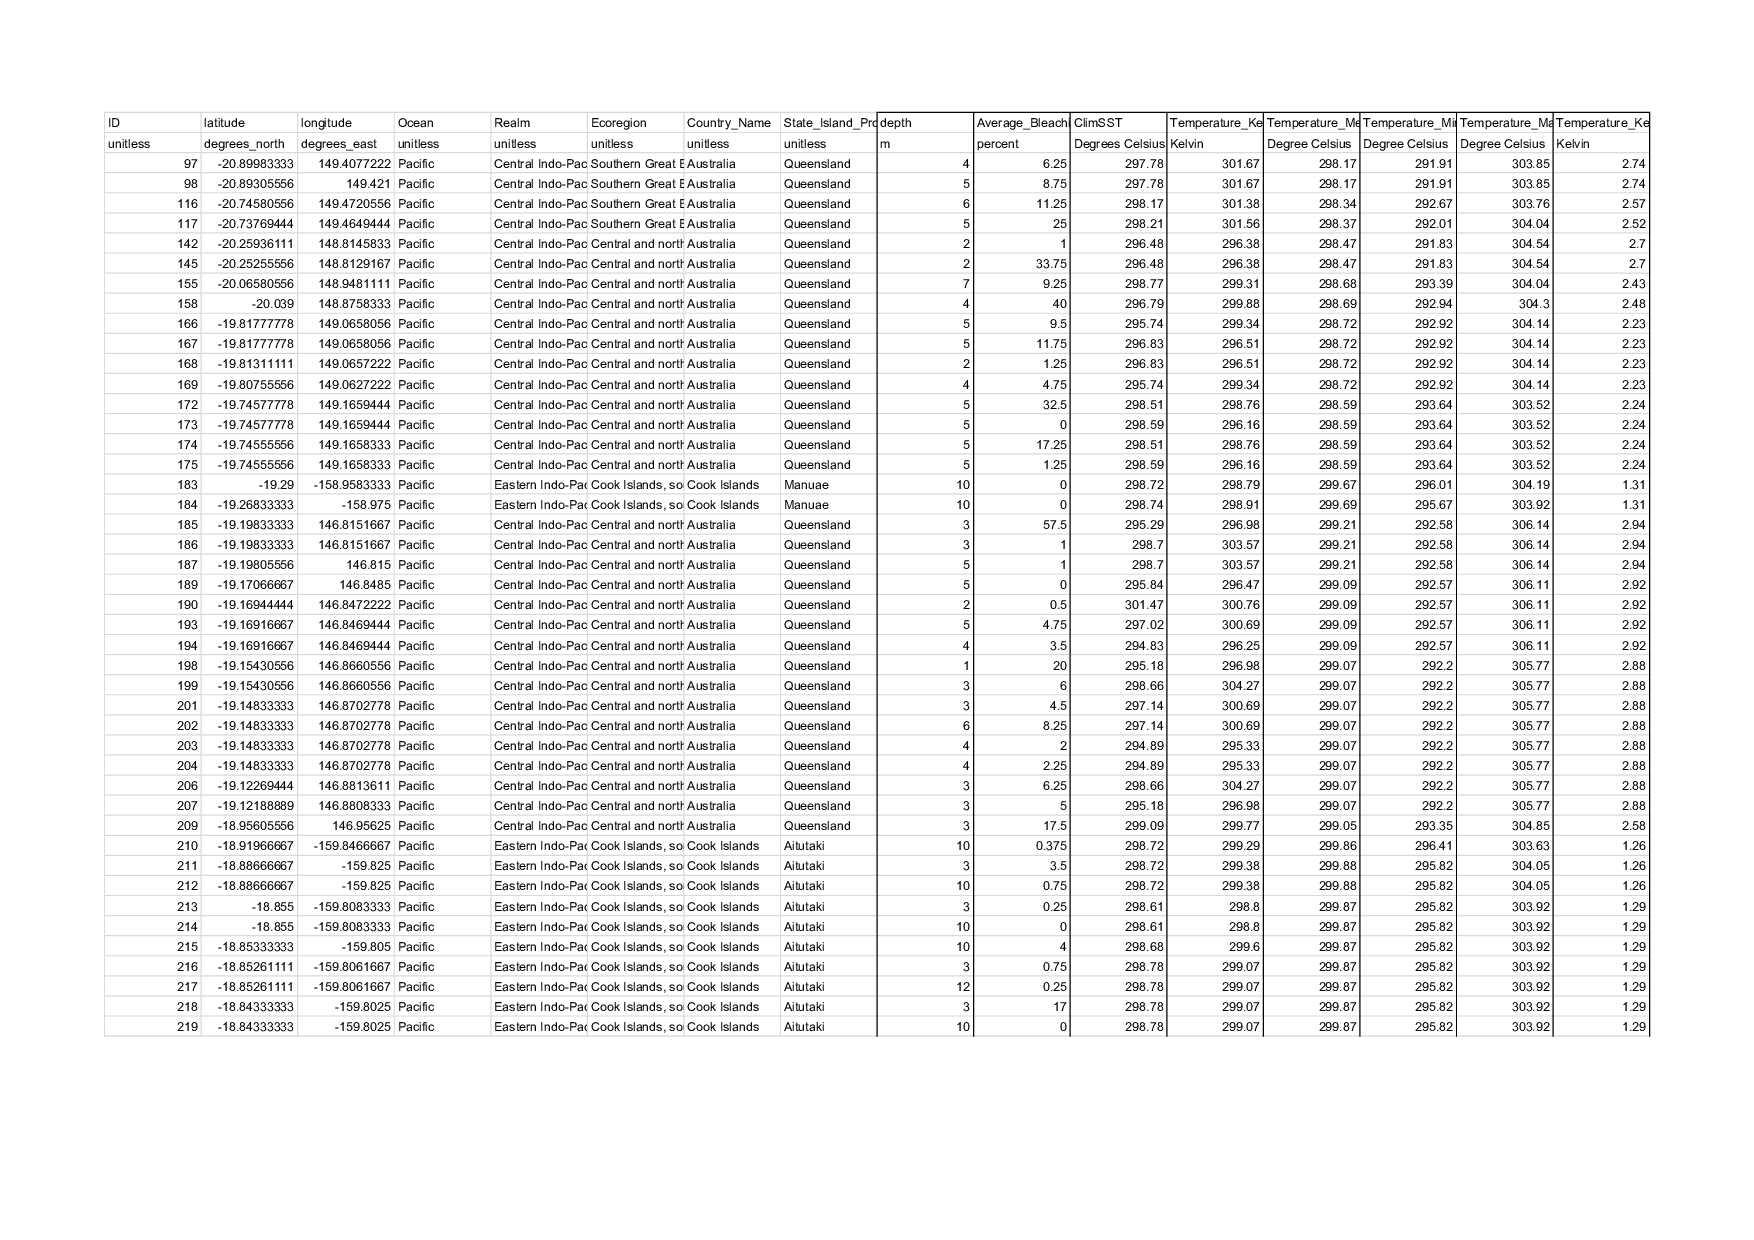
\includegraphics[height=0.6\textheight]{dataset_coral.png}
	\caption{Representación de la información guardada en la base de datos.}
	\label{fig: tabla}
\end{figure}

	
\newpage
\subsection{Muestreo}

	\par Tenemos una base datos con $10,000$ entradas, estas serán tomadas como la población sobre la cual queremos sacar una muestra. Si tomamos los siguientes parámetros
	\begin{itemize}
		\item Margen: 10\%
		\item Nivel de confianza: 99\%
		\item Poblacion: 10000
	\end{itemize}
	
	\noindent y con la fórmula que revisamos en el curso; obtenemos que el tamaño ideal de la muestra debe ser 163.

	
	\begin{figure}[h]
	\centering
		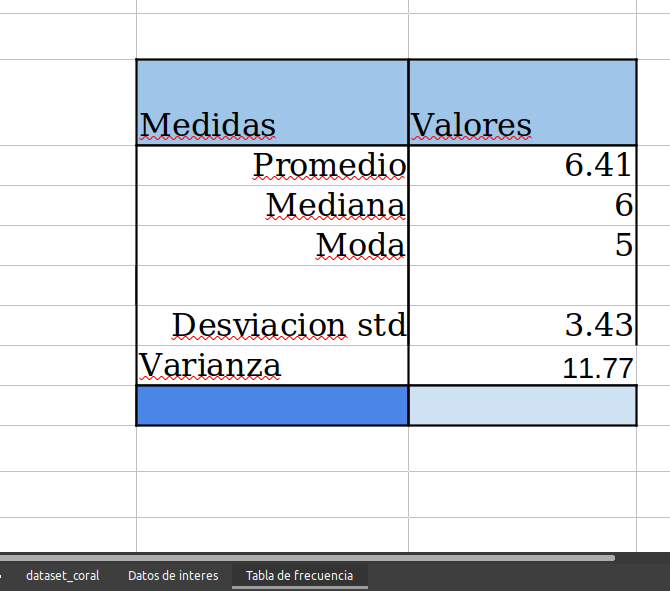
\includegraphics[width=0.7\textwidth]{medidas-EA-U3.png}
	\caption{Medidas de dispersión y tendencia central.}
	\label{fig: tabla frecuencia}
\end{figure}

	

\subsection{Medidas de dispersión y tendencia central}

	\par En la figura~\ref{fig: tabla frecuencia} están expresadas las medidas de tendencia central y dispersión, que revisamos en esta unidad, que fueron obtenidas de la muestra de la población. La muestra fue obtenida con ayuda de la funcion \textit{muestra} de \textbf{Excel} y esta en otro libro porque son bastante datos.
	\par De los datos podemos notar que el promedio y la mediana son bastante parecidas; esto implica que los datos estan parcialmente bien distribuidos, solo algo cargados en el percentil inferior. Aunque por otro lado, el que la moda no coincida con estos indica que hay valores \textit{erráticos} en ambos extremos de los datos.
	\par En otro análisis identificamos que la máxima profundidad registrada es $21.7$, mientras que la mínima es $0.1$.
	


\subsection*{Obtención de datos}

	\par En este trabajo se trabajo sobre el promedio, la mediana, la moda, la desviación estandar y la varianza. A continuación trataremos de definir estas variables y de explicar como podemos obtenerlas.
	
	\begin{description}
		\item [Promedio] Este se define como el \textit{valor característico de una serie de datos cuantitativos}. Este se obtiene al dividir la sumatoria de todos los datos y dividirlos entre la cantidad de datos $n$ que se tienen.
			$$ \text{promedio} = \bar x = \frac{\sum x_i}{n}$$
			
			Para esto usamos la función \texttt{PROMEDIO} de excel, al cual sólo se le pasa el rango de los datos a promediar.
			
		\item [Mediana] Por otro lado, esta representa el valor de la variable de posición central en un conjunto de datos ordenados; de manera que hay la misma cantidad de datos de ambos lados que esta entrada. En caso de que haya una cantidad par de datos, se saca un promedio de los dos datos centrales.
			
			Esto también tiene una función en excel, \texttt{MEDIANA}. También sólo se le pasa el rango de los datos para sacar la mediana.
		
		\item [Moda] Es el valor con mayor frecuencia en la distribucion de datos. Esta es la única medida de tendencia central que se puede obtener para datos cualitativos y cuantitativos.
		
			Para esta sigue extiendo una fórmula ya definida en excel. Para la función \texttt{MODA} recibe los datos de los que se quiere obtener la moda.
		
		\item [Desviación estandar] Es una medida de dispersión que se utiliza para cuantificar la variación o la dispersión de un conjunto de datos numéricos. La función en excel que la calcula es \texttt{STDEV} y recibe el rango de los datos a medir.
		
		\item [Varianza] Es una medida de dispersión que representa la variabilidad de una serie de datos respecto a su media. En excel se puede calcular de dos formas, como el cuadrado de la desviación estandar; o con la función \texttt{VAR}.
	\end{description}




\section{Conclusiones}

	\par Todas estas medidas y cálculos, que revisamos en la unidad, no permiten entender la manera en que los datos están esparcidos en el espacio. Sin estas herramientas deberíamos de tener la capacidad de leer los datos individualmente y tener la habilidad para contextualizar y recordar cada uno de los detalles de los datos. Por todo esto, podemos concluir que estos cálculos definitivamente son útiles cuando se debe trabajar con grandes cantidades de datos cuantitativos.
	\par Me parece que sería ideal que nos dieran más casos específicos y ejercicios en esta sección, esto nos permitiría entender mejor estos temas.



%%%%%%%%%%%%%%%%%%%%%%%%%%%%%%%%
%%         Bibliografia        %%
%%%%%%%%%%%%%%%%%%%%%%%%%%%%%%%%%%

\begin{thebibliography}{X}
	\bibitem{EA anterior} Rivera C., B. (2020). \textit{Evidencia de Aprendizaje U2}. No Publicado.
	\bibitem{basico} Universidad Abierta y a Distancia de México. (s/f). \textit{Unidad 3. Representación numérica y gráfica de datos}. UnADM.
	\bibitem{db} van Woesik, R. (2019). \textit{Dataset: Global Bleaching and Environmental Data [Base de Datos]}. Florida Institute of \url{Technology. https://www.bco-dmo.org/dataset/773466}
 
\end{thebibliography}

\end{document}